\problemname{Kitchen Cable Chaos}

You started your new project: installing a home automation system. You already bought all the components and in your local electronic shop you found a promotion set with a bunch of cables of different lengths.
Now you want to connect your controller with your smart sandwich maker that is several meters away, but you are lacking a cable that is long enough.

To solve this problem you have to connect some of your cables to form a long one.
You measure the lengths of every cable you own. Exactly 5 centimeters of isolation are stripped on both ends of every cable. To connect two cables, you overlap and twist the stripped ends. It is enough for the cables to touch each other with an overlap of 0. You cannot have an overlap of more than 5 centimeters, but the connection quality increases with longer overlaps. On both ends -- the controller and the sandwich maker -- you also have 5 centimeters of stripped end, to which you have to connect your newly created cable in the same way.
The connection quality of your link is determined by the smallest overlap used and your goal is to maximize this value.

The problem would be really easy, but your perfectionist roommate hates unnecessary use of cables. Therefore, the cable has to form a straight line, without any loops or detours. And cutting the cables is no option, obviously.

\begin{figure}[!h]
  \centering
  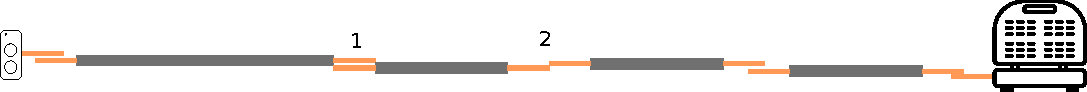
\includegraphics[width=.80\textwidth]{wires}
  \caption{Four cables of different lengths connect the controller with the sandwich maker, with different overlaps. Connection 1 has the maximal overlap, connection 2 the minimal overlap and all other connections are in between. The quality of this setup is 0.}
\end{figure}

Considering all possible arrangements of cables, find the one with the best quality.

\section*{Input}

The input consists of:
\begin{itemize}
  \item one line with two integers $n,g$ ($1 \le n \le 60$, $11 \le g \le 1\,000$), the number of cables and the distance to be covered in centimeters,
    measured between the casings of the controller and the sandwich maker;
  \item $n$ lines, each with an integer $d$ ($11 \le d \le 1\,000$),
    giving the lengths of the cables (including the stripped ends).
\end{itemize}

Each of the $n$ cables can be used at most once.

\section*{Output}
Output one number, the best achievable quality. The quality must be accurate up to a relative or absolute error (whichever is lower) of $10^{-7}$. If no arrangement fits your needs, output \texttt{impossible}.
